\section{Implementation and Evaluation}

We have implemented our prototype, called \doccam,
using \occam~\cite{occam}. The architecture of \doccam is depicted in
\cref{fig:d-occam}.
%
\doccam takes as inputs a set of LLVM modules (main application and
libraries) and a manifest (i.e., a user-defined execution environment)
and produces a specialized binary.
%
We used Gadget Set Analyzer (\gsa)~\cite{gsa} to evaluate 
 the specialized binary and
\pytorch~\cite{pytorch} for training the deep learning~models. % The communication between \occam and \pytorch is via gRPC
 
% channels.
At each call-site, \occam calculates the features
described in \cref{tab:features} from the \llvm module, sending them to the \pytorch server, and
transforming the code based on the returned decision.
%
During inference, the \pytorch server receives the message and runs the learnt
policy to decide whether to specialize that
call-site. During training, the \pytorch server also keeps track of all the
decisions it has made and uses that information to update its
policy. We run multiple copies of \occam on multiple copies of the \pytorch
server to scale up the learning process, which is justified by the Markov property of the state.%  sumed, we can easily
% run multiple copies of \occam on multiple codebases at the same time with just a
% single \pytorch server: to pick the action for a call-site, the server
% needs exactly one message from \occam. Hence, we do not have to keep
% track of where the messages are coming from and their history.


%% \subsection{Implementation details}
%% In order to implement our pipeline, we need two building blocks: one for
%% analyzing and interacting with the source code, and one for training
%% and using deep learning models. We choose to use LLVM \cite{llvm} for the former part,
%% and PyTorch \cite{pytorch} for the latter. Furthermore, we need a communication layer between
%% them. We chose gRPC for its simplicity and performance. 

%% We build our framework on top of \emph{OCCAM} \cite{occam}. The architecture is depicted in Figure
%% ~\ref{fig:d-occam}.

%% gRPC channels are added to \occam to communicate with the PyTorch server. At each call-site, \occam is
%% responsible for profiling the module to extract the 4 vectors mentioned in
%% Section~\ref{subsec:asr}, sending them to the PyTorch server, and transforming the code
%% based on the returned decision.

%% During inference, the PyTorch server receives the
%% message, runs the learnt policy to decide whether or not \occam should specialize
%% that call-site. During training, the PyTorch server also keeps track of all the
%% decisions it has made, and use that information to update its policy. With the
%% Markov property of the state assumed, we can easily run multiple \occam on multiple
%% codebases at the same time with just a single PyTorch server: to pick the
%% action for a call-site, the server needs exactly one message from \occam. Hence,
%% we do not have to keep track of where the messages are coming from and their history.

%%%%%%%%%%%%%%%%%%%%%%%%%%%%%%%%%%%%%%%%%%%%%%%%%%%%%%%%%%%%%%%%%%%%%%%%%%%%%%%%%%%%%%%%%%%%%%%%%%%%%%%
% The architecture allows great scalability and helps us utilize the right                            %
% hardware for the right job: the Core should be run on machines with strong CPUs,                    %
% while the PyTorch server should be run on machines with strong GPUs. The server could be            %
% written in any deep learning framework to make use of open source                                   %
% implementations of state-of-the-art learning algorithms. While both PyTorch and TensorFlow have C++ %
% bindings, they are not as well supported and documented as their Python counterparts.               %
%%%%%%%%%%%%%%%%%%%%%%%%%%%%%%%%%%%%%%%%%%%%%%%%%%%%%%%%%%%%%%%%%%%%%%%%%%%%%%%%%%%%%%%%%%%%%%%%%%%%%%%

\begin{figure}
     \centering
     \begin{subfigure}[b]{0.4\textwidth}
         \centering
         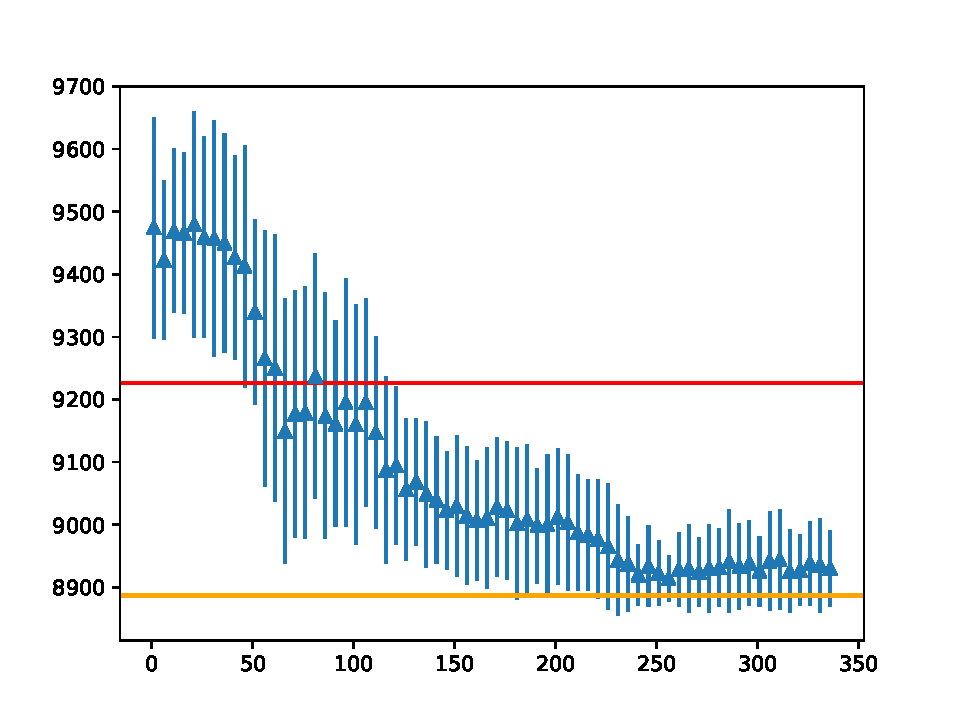
\includegraphics[width=\textwidth]{doccam_figures/tree_hf_lr_0001/Number_of_instructions_75_339_sparsed.pdf}
         \label{fig:inst}
         \vspace{-0.2in}
         \caption{Instructions (\textbf{HF})}
       \end{subfigure}
     \begin{subfigure}[b]{0.4\textwidth}
         \centering
         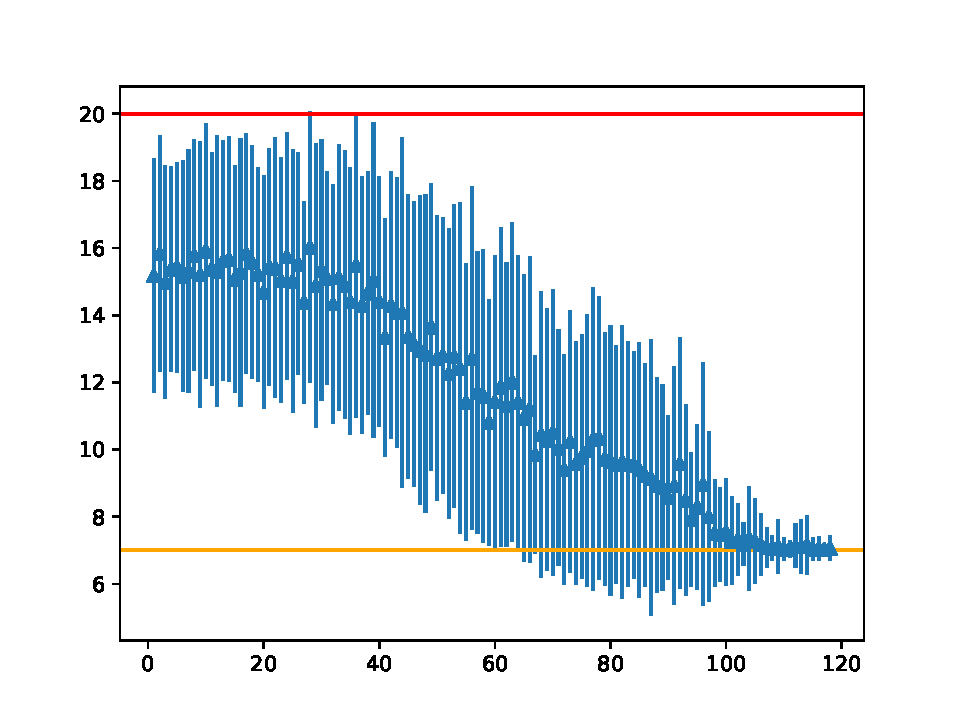
\includegraphics[width=\textwidth]{doccam_figures/tree_hf_lr_0001/COP_gadgets_75_119.pdf}
         \label{fig:cop}
         \vspace{-0.2in}
         \caption{COP gadgets (\textbf{HF})}
       \end{subfigure}
       \begin{subfigure}[b]{0.4\textwidth}
         \centering
         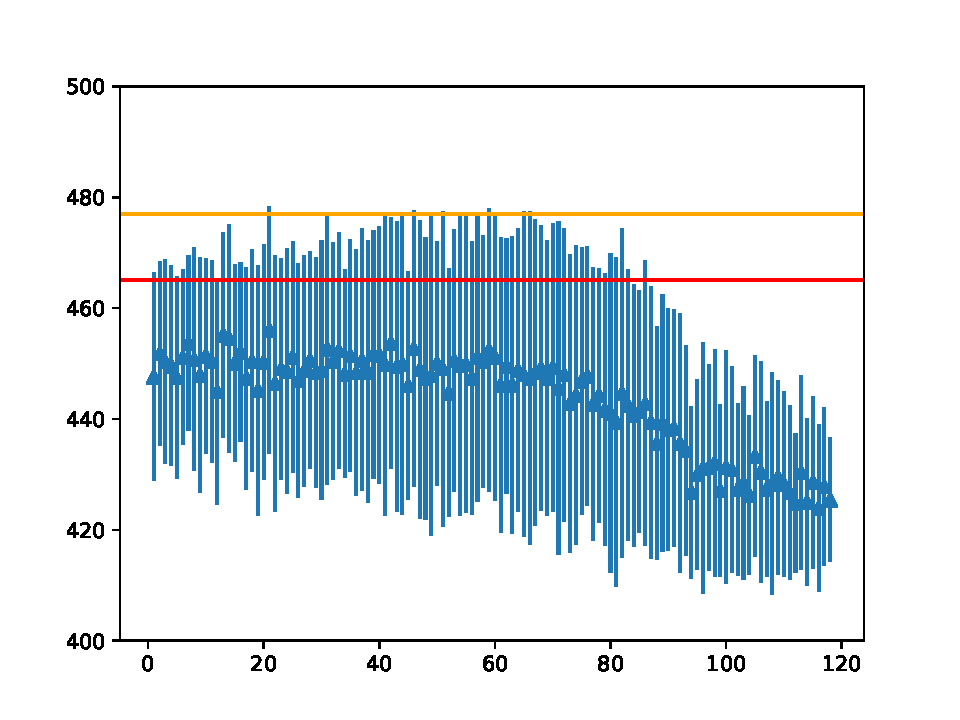
\includegraphics[width=\textwidth]{doccam_figures/tree_hf_lr_0001/ROP_gadgets_75_119_sparsed.pdf}
         \label{fig:rop}
         \vspace{-0.2in}
         \caption{ROP gadgets (\textbf{HF})}
     \end{subfigure}
     \begin{subfigure}[b]{0.4\textwidth}
         \centering
         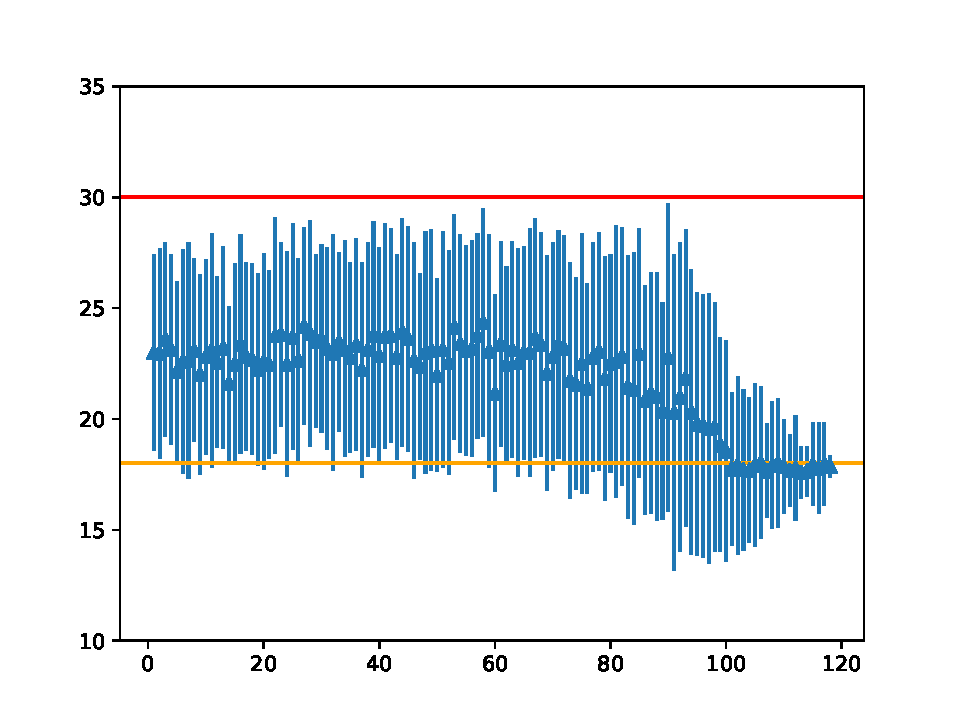
\includegraphics[width=\textwidth]{doccam_figures/tree_hf_lr_0001/JOP_gadgets_75_119_sparsed.pdf}
         \label{fig:jop}
         \vspace{-0.2in}
         \caption{JOP gadgets (\textbf{HF})}
     \end{subfigure}
     \begin{subfigure}[b]{0.4\textwidth}
         \centering
         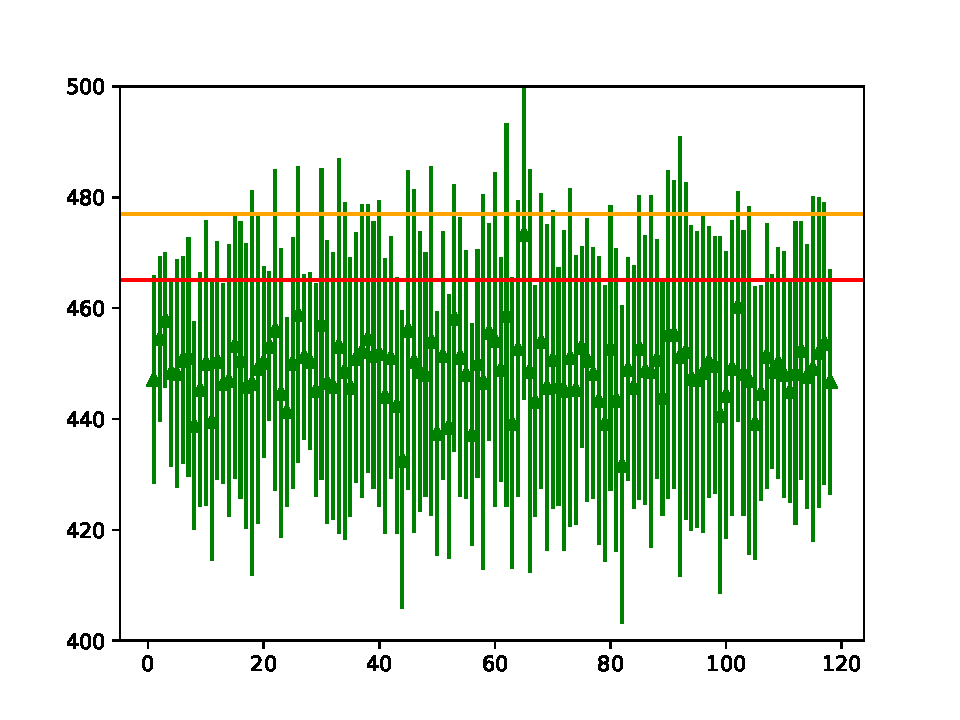
\includegraphics[width=\textwidth]{doccam_figures/tree_iv_lr_0001/ROP_gadgets_20_119_sparsed.pdf}
         \label{fig:inst2vec_rop}
         \vspace{-0.2in}
         \caption{ROP gadgets (\textbf{IV})}
       \end{subfigure}
  \begin{subfigure}[b]{0.4\textwidth}
         \centering
         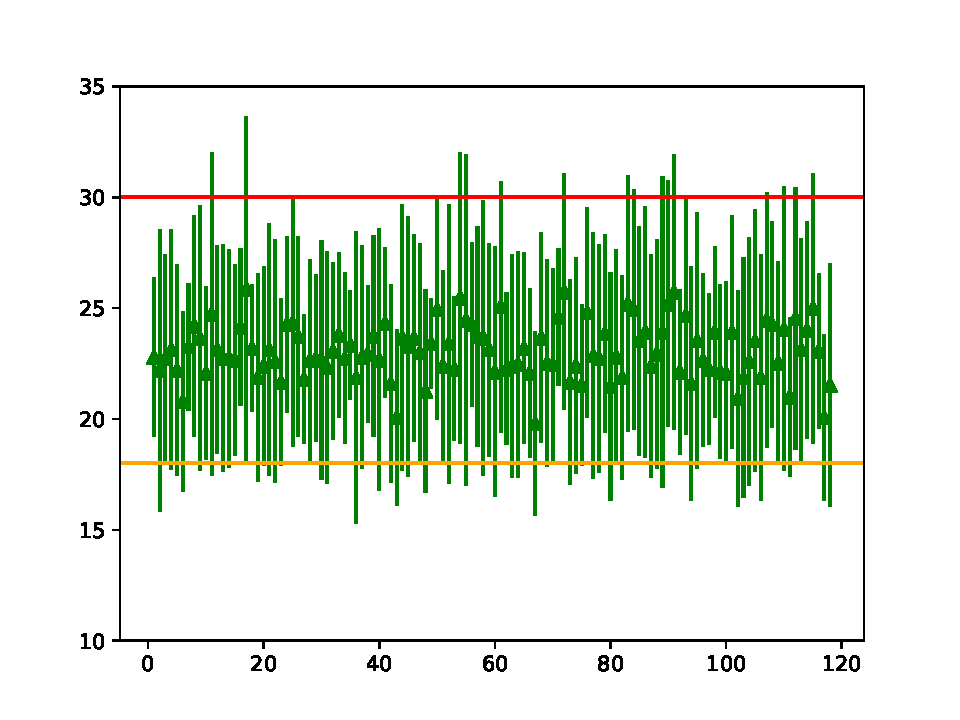
\includegraphics[width=\textwidth]{doccam_figures/tree_iv_lr_0001/JOP_gadgets_15_119_sparsed.pdf}
         \label{fig:inst2vec_inst}
         \vspace{-0.2in}
         \caption{JOP gadgets (\textbf{IV})}
       \end{subfigure}
       \caption{
Results for optimizing different metrics using \textbf{HF} and \textbf{IV}. x-axis is the number
of RL iterations. y-axis is the results. Dots and bars are mean and std. dev. of
$k$ runs in each iteration. \textbf{HF} results are in blue while
\textbf{IV} results are in green. Orange and red lines are \occamo and \occama results, respectively.}
     \label{fig:results}
     \end{figure}



We compare \doccam with \occam running in two modes.
%
First, \occama that runs \occam with a
\emph{nonrecursive-aggressive} policy. This always specializes a
call-site if the callee is not a recursive function.
%
Second, \occamo that runs \occam without specializing any call-site.
%
Fig.~\ref{fig:results} shows the comparision between \doccam using \textbf{HF}
, \doccam using \textbf{IV}, \occama , and \occamo for debloating \gnutree. 
% \nl{discuss the graphs}
On average, \doccam outperforms both \occamo and \occama in reducing the number of
ROP and JOP gadgets, matches \occamo on COP gadgets, and underperforms 
in reducing the number of instructions. Interestingly, while \doccam matches
\occamo on COP, it finds a different policy that specialize some call-sites.
For optimizing the number of instructions, we run 200 more training iterations
but are not able to outperform \occamo. We include the results for the number of
instructions only to demonstrate the flexibility of our approach.
% vNote that optimizing the number of instructions is not our main target, since \doccam relies
% n \llvm to perform other code transformation passes, and \llvm also
% has its own heuristics controlling those passes to reduce the size of the final
% binary. The results for optimizing the number of instructions are included just to
% demonstrate the flexibility of our approach

% \nl{why inst2vec is not working}
In all of our experiments, the learning procedure does not converge when we use
\insttovec pre-trained embedding. Upon closer inspection, we observe that
the software in our test suite, once compiled to LLVM IR, contained many
instructions regarded as low-frequency by \insttovec. Consequently, they are all
mapped into the same \texttt{UNK!} token in the cutoff dictionary. Hence, the
calling context window that we use suffers from the state aliasing problem: different
calling contexts are mapped to the same vector of tokens. 

This is surprising since \insttovec claims to train the embedding on a wide
range of software written in C, C++, FORTRAN, and OpenCL, specifically to avoid overfitting
to a small family of code bases.

%%% Local Variables:
%%% mode: latex
%%% TeX-master: "neurips_2019"
%%% End:
